\documentclass[a4paper,fleqn]{cas-sc}
\usepackage[authoryear]{natbib}
\usepackage{lineno}
\usepackage{booktabs}
\usepackage{url}
\linenumbers

\begin{document}
\let\WriteBookmarks\relax
\def\floatpagepagefraction{1}
\def\textpagefraction{.001}

\shorttitle{Resposta da fotossíntese líquida às fases do ENSO}
\shortauthors{Y.A.S. Oliveira et al.}

\title[mode = title]{Resposta assimétrica da fotossíntese líquida MODIS às fases do ENSO ao longo de um gradiente hidroclimático tropical: Mata Atlântica, Cerrado e Caatinga (Bahia, Brasil), 2001--2025}

\author[1]{Ygor Augusto dos Santos Oliveira}[orcid=0009-0001-5821-658X]
\cormark[1]
\ead{ygornayty2@gmail.com}
\credit{Conceituação, Metodologia, Software, Análise formal, Curadoria de dados, Redação -- rascunho original}

\author[1]{Nayanne Silva Benfica}
\credit{Conceituação, Metodologia, Curadoria de dados, Redação -- revisão e edição, Supervisão}

\author[1]{Fabr\'icio Berton Zanchi}[orcid=0000-0002-8074-2893]
\credit{Conceituação, Metodologia, Redação -- revisão e edição, Supervisão}

\affiliation[1]{organization={Programa de Pós-graduação em Ciências e Tecnologias Ambientais, Universidade Federal do Sul da Bahia / Instituto Federal de Educação, Ciência e Tecnologia da Bahia},
  city={Porto Seguro},
  postcode={45810-000},
  state={Bahia},
  country={Brasil}}

\cortext[1]{Autor correspondente}

\begin{abstract}
O El Niño--Oscilação Sul (ENSO) modula a produtividade da vegetação tropical por meio de variáveis climáticas intermediárias, mas a forma dessa modulação depende do regime ecológico de cada bioma. Este trabalho caracterizou a resposta da fotossíntese líquida (PSN, MOD17A2HGF) às fases do ENSO em três biomas dispostos ao longo de um gradiente hidroclimático no Nordeste do Brasil, entre 2001 e 2025, com 297 períodos mensais por bioma. As anomalias mensais, obtidas pela remoção do ciclo anual, foram comparadas entre as fases oficiais da NOAA, e a fração da resposta transmitida pelo clima regional foi estimada impondo-se as anomalias médias de cada fase a um modelo de regressão polinomial regularizada ajustado aos mesmos dados. A resposta foi assimétrica e específica de cada bioma: a Mata Atlântica respondeu à fase quente, com redução média de 5,4~p.p.\ na PSN e aumento da frequência de meses extremamente baixos de 4,7\% para 22,4\%, acompanhando um aquecimento da superfície de 3,1~p.p.\ (cerca de 0,9~$^{\circ}$C); o Cerrado e a Caatinga responderam à fase fria, com aumentos de 11,7 e 10,4~p.p., acompanhados de anomalias positivas de evapotranspiração e de disponibilidade hídrica. A precipitação do próprio mês não diferiu entre fases em nenhum bioma. O modelo reproduziu de 57\% a 94\% da magnitude observada, pela via térmica no bioma úmido e pela evapotranspiração nos sazonais, e a defasagem de maior correlação variou de zero meses na Caatinga a dez no Cerrado. Nenhum bioma apresentou tendência interanual significativa. Uma verificação de robustez em que a unidade amostral passa do mês para o episódio --- os 76 meses de El Niño correspondem a 8 episódios e os 72 de La Niña a 9 sequências --- alarga os intervalos de confiança em 1,67 vez em mediana e reduz de 10 para 3 o número de efeitos distinguíveis de zero, entre os quais permanecem a resposta da Mata Atlântica ao El Niño e a da Caatinga à La Niña. O padrão assimétrico é consistente entre as duas análises, mas a magnitude dos efeitos é estimada com precisão limitada pelo pequeno número de episódios disponíveis em 24 anos.
\end{abstract}

\begin{keywords}
El Niño--Oscilação Sul \sep fotossíntese líquida \sep MODIS \sep Caatinga \sep Cerrado \sep bootstrap em blocos
\end{keywords}

\maketitle

\section{Introdução}

O El Niño--Oscilação Sul (ENSO) é o principal modo de variabilidade interanual do sistema climático e organiza boa parte das anomalias de precipitação e de temperatura da América do Sul \citep{ropelewski1987, trenberth1997, grimm2003, grimm2009, cai2020}. No Nordeste do Brasil, episódios quentes costumam ser associados a redução das chuvas e episódios frios a chuvas acima da média, com intensidade que varia conforme a estação e a posição geográfica \citep{kayano2007, marengo2018}. Como a produtividade da vegetação tropical responde à disponibilidade de água e à demanda evaporativa, é esperado que essa variabilidade climática se propague para os fluxos de carbono \citep{zhao2010, nemani2003}.

Essa propagação, porém, não é direta. O ENSO não atua sobre a vegetação: atua sobre a temperatura, a precipitação e o balanço hídrico regionais, e são essas variáveis que condicionam a assimilação de carbono. Daí decorre que biomas submetidos ao mesmo forçante remoto possam responder de maneiras distintas, conforme o fator que limita sua produtividade. Em sistemas limitados pela água, um excedente hídrico durante a fase fria tende a elevar a produtividade; em sistemas úmidos, em que a água raramente é limitante, o efeito relevante tende a ser o estresse térmico e evaporativo da fase quente. A expectativa, portanto, não é de uma resposta única, mas de respostas assimétricas entre fases e entre biomas.

O estado da Bahia oferece um contexto favorável para examinar essa assimetria. Em cerca de 565 mil km$^2$ reúne três biomas dispostos ao longo de um gradiente hidroclimático contínuo, da Mata Atlântica úmida no litoral à Caatinga semiárida no interior, com o Cerrado na posição intermediária \citep{ibge2019, alvares2013}. Os três compartilham o mesmo forçante remoto e o mesmo protocolo de extração de dados, o que permite comparar respostas sem confundir bioma com metodologia. A produtividade desses biomas e sua relação com fatores climáticos e antrópicos já foi descrita para a região \citep{benfica2022, benfica2023}, e um modelo de regressão polinomial regularizada da PSN mensal foi desenvolvido e validado para os mesmos três biomas e o mesmo período \citep{oliveira2026}, o que permite estimar quanto de uma resposta observada o clima medido é capaz de reproduzir.

Este trabalho caracteriza a resposta da fotossíntese líquida às fases do ENSO nos três biomas, quantifica a defasagem dessa resposta e a fração dela transmitida pelas variáveis climáticas intermediárias, e examina a escala anual. Por fim, submete os resultados a uma verificação de robustez pouco usual em estudos dessa natureza: como os meses de uma mesma fase pertencem a um número reduzido de episódios e são fortemente autocorrelacionados, toda a análise é repetida tomando o episódio, e não o mês, como unidade amostral \citep{kunsch1989, politis1994}.

\section{Material e métodos}

\subsection{Área de estudo}

A área compreende as porções baianas da Mata Atlântica, do Cerrado e da Caatinga, delimitadas pelo mapa de biomas do IBGE na escala 1:250.000 recortado pelo limite estadual \citep{ibge2019}. O gradiente hidroclimático vai de Af/Am no litoral a BSh no interior semiárido, com precipitação média anual de cerca de 1.400~mm na Mata Atlântica, 1.000~mm no Cerrado e 600~mm na Caatinga \citep{alvares2013}. A descrição detalhada dos biomas e do protocolo de extração consta de \citet{oliveira2026}.

\subsection{Dados}

A série mensal cobre janeiro de 2001 a setembro de 2025, com 297 períodos por bioma. Cada período é uma janela fixa de quatro compósitos consecutivos de oito dias, atribuída ao mês civil que contém a maior parte de seus dias. A fotossíntese líquida (PSN) provém do MOD17A2HGF C6.1 \citep{running2021gpp}; a evapotranspiração real (EV) e a potencial, do MOD16A2GF C6.1 \citep{running2021et}; a temperatura diurna da superfície (TST), do MOD11A2 C6.1 \citep{wan2021}; e a precipitação (PRE), do GPM IMERG Final Run V07 \citep{huffman2023}. O índice de disponibilidade hídrica (WAI) é a razão entre evapotranspiração real e potencial. As médias espaciais foram calculadas sobre os pixels válidos de cada bioma no Google Earth Engine \citep{gorelick2017}.

O Índice Oceânico Niño (ONI) foi obtido da tabela completa do Climate Prediction Center da NOAA \citep{noaacpc2025}. A classificação das fases segue o critério oficial: El Niño quando o ONI permanece em $+0{,}5$~$^{\circ}$C ou acima por cinco trimestres consecutivos sobrepostos, La Niña quando permanece em $-0{,}5$~$^{\circ}$C ou abaixo pelo mesmo intervalo, e Neutro nos demais casos. A série completa do índice desde 1950 foi usada na classificação, de modo que episódios iniciados antes de 2001 fossem reconhecidos.

\subsection{Anomalias}

Para cada variável e bioma, a climatologia é a média do mês civil correspondente ao longo de toda a série, e a anomalia é expressa em porcentagem dessa média. A remoção do ciclo anual é necessária porque as fases do ENSO não se distribuem uniformemente pelo calendário: os meses de El Niño representam de 10,5\% a 11,8\% da amostra entre novembro e fevereiro, mas apenas de 3,9\% a 5,3\% entre maio e julho, ao passo que os meses neutros seguem a distribuição inversa (4,0\% e 12,8\%, respectivamente). Uma comparação sobre valores brutos confundiria, portanto, fase e estação.

\subsection{Comparação entre fases}

A anomalia de cada fase ativa foi comparada à dos meses neutros pelo teste de Mann-Whitney, e as três fases pelo teste de Kruskal-Wallis, com o tamanho de efeito $\varepsilon^2$. A homogeneidade da dispersão foi avaliada pelo teste de Fligner-Killeen e a frequência de extremos por um teste qui-quadrado sobre a proporção de meses abaixo do percentil 10 e acima do percentil 90 da própria série de anomalias. Os valores de $p$ de cada família de testes foram corrigidos pelo procedimento de Benjamini-Hochberg, controlando a taxa de falsas descobertas em 5\% \citep{benjamini1995}.

\subsection{Defasagem}

A resposta defasada foi avaliada pela correlação de Spearman entre o ONI do mês $t$ e a anomalia de PSN do mês $t+L$, para $L$ de 0 a 12 meses. Por serem fortemente correlacionadas entre si, as defasagens não foram submetidas a correção para comparações múltiplas e são lidas como descrição do padrão temporal, não como testes independentes.

\subsection{Mediação pelo modelo climático}

Para estimar que fração da resposta da PSN é reproduzida pelas variáveis climáticas medidas, usou-se o modelo de regressão polinomial de grau 2 com regularização de Ridge ajustado para os mesmos biomas e período \citep{oliveira2026, hoerl1970}. O modelo foi usado para prever a PSN com os preditores em sua climatologia mensal e, alternativamente, com cada preditor --- ou todos --- deslocado pela anomalia média observada em cada fase; a diferença entre as duas predições, em porcentagem da PSN climatológica, é a parcela da resposta atribuível a cada canal no modelo. Trata-se de uma decomposição baseada no modelo, sem pretensão de inferência causal.

\subsection{Variabilidade interanual}

A PSN anual é a soma dos períodos de cada ano. A tendência foi estimada pelo declive de Sen \citep{sen1968} e testada por Mann-Kendall \citep{mann1945}, com intervalo de confiança por bootstrap. A soma anual foi comparada, por correlação de Pearson, ao NPP anual do produto MOD17A3HGF para as mesmas máscaras de bioma, como verificação de consistência entre dois produtos da mesma família. O ano de 2025, com nove períodos disponíveis, foi excluído do cálculo de tendência.

\subsection{Verificação de robustez: o episódio como unidade amostral}

Os testes descritos na Seção~2.4 supõem que as observações de cada grupo sejam independentes. Os meses de uma mesma fase não o são: pertencem a um número reduzido de episódios, cada um com vários meses consecutivos, e tanto o forçante oceânico quanto a resposta da vegetação são autocorrelacionados dentro de um episódio. A unidade efetiva de amostragem é o episódio.

Para medir o efeito dessa distinção, a estatística de interesse --- a diferença entre a anomalia percentual média de uma fase ativa e a dos meses neutros --- foi acompanhada de dois intervalos de confiança de 95\%, ambos por percentis de 10.000 reamostragens com a mesma semente: um por bootstrap i.i.d., sorteando meses com reposição dentro de cada grupo, que é o esquema implícito nos testes convencionais; e outro por bootstrap em blocos, sorteando com reposição sequências contíguas inteiras de meses da mesma fase \citep{kunsch1989, politis1994}, o que preserva a dependência interna de cada episódio. Os blocos foram definidos como corridas contíguas de meses na mesma fase oficial, sem imposição de comprimento: cada bloco é um episódio do ENSO tal como a NOAA o delimita. Os dois esquemas foram aplicados à PSN e aos quatro preditores nos três biomas, totalizando 30 testes.

Todas as análises foram feitas em Python 3.11 com \texttt{numpy}, \texttt{pandas}, \texttt{scipy} e \texttt{scikit-learn}.

\section{Resultados}

\subsection{Composição das fases}

Dos 297 períodos da série, 76 foram classificados como El Niño, 72 como La Niña e 149 como neutros. Esses meses distribuem-se em poucas sequências contíguas: 8 episódios de El Niño, 9 sequências de La Niña --- uma das quais truncada no início da série, em janeiro e fevereiro de 2001 --- e 17 intervalos neutros (Tabela~\ref{tab:fases}), com duração entre 2 e 20 meses e mediana de 8 meses.

\begin{table}[width=\linewidth,cols=5,pos=h]
\caption{Composição das fases do ENSO na série mensal de 2001 a 2025, segundo o critério oficial da NOAA.}
\label{tab:fases}
\begin{tabular*}{\tblwidth}{@{}lrrrr@{}}
\toprule
Fase & Meses & Sequências & \multicolumn{2}{c}{Duração (meses)} \\
\cmidrule(l){4-5}
 & & & mediana & mín--máx \\
\midrule
El Niño & 76  & 8  & 8,5 & 5--20 \\
Neutro  & 149 & 17 & 7   & 1--30 \\
La Niña & 72  & 9  & 7   & 2--17 \\
\midrule
Total   & 297 & 34 & --- & --- \\
\bottomrule
\end{tabular*}
\end{table}

A Figura~\ref{fig:episodios} mostra a série de anomalias de PSN dos três biomas com os episódios sombreados. A variabilidade mensal é alta em todos os biomas --- amplitude de cerca de $\pm 40\%$ na Mata Atlântica e de $\pm 90\%$ no Cerrado --- e o El Niño de 2014--2016 coincide com as anomalias negativas mais profundas da Mata Atlântica.

\begin{figure}[pos=h]
\centering
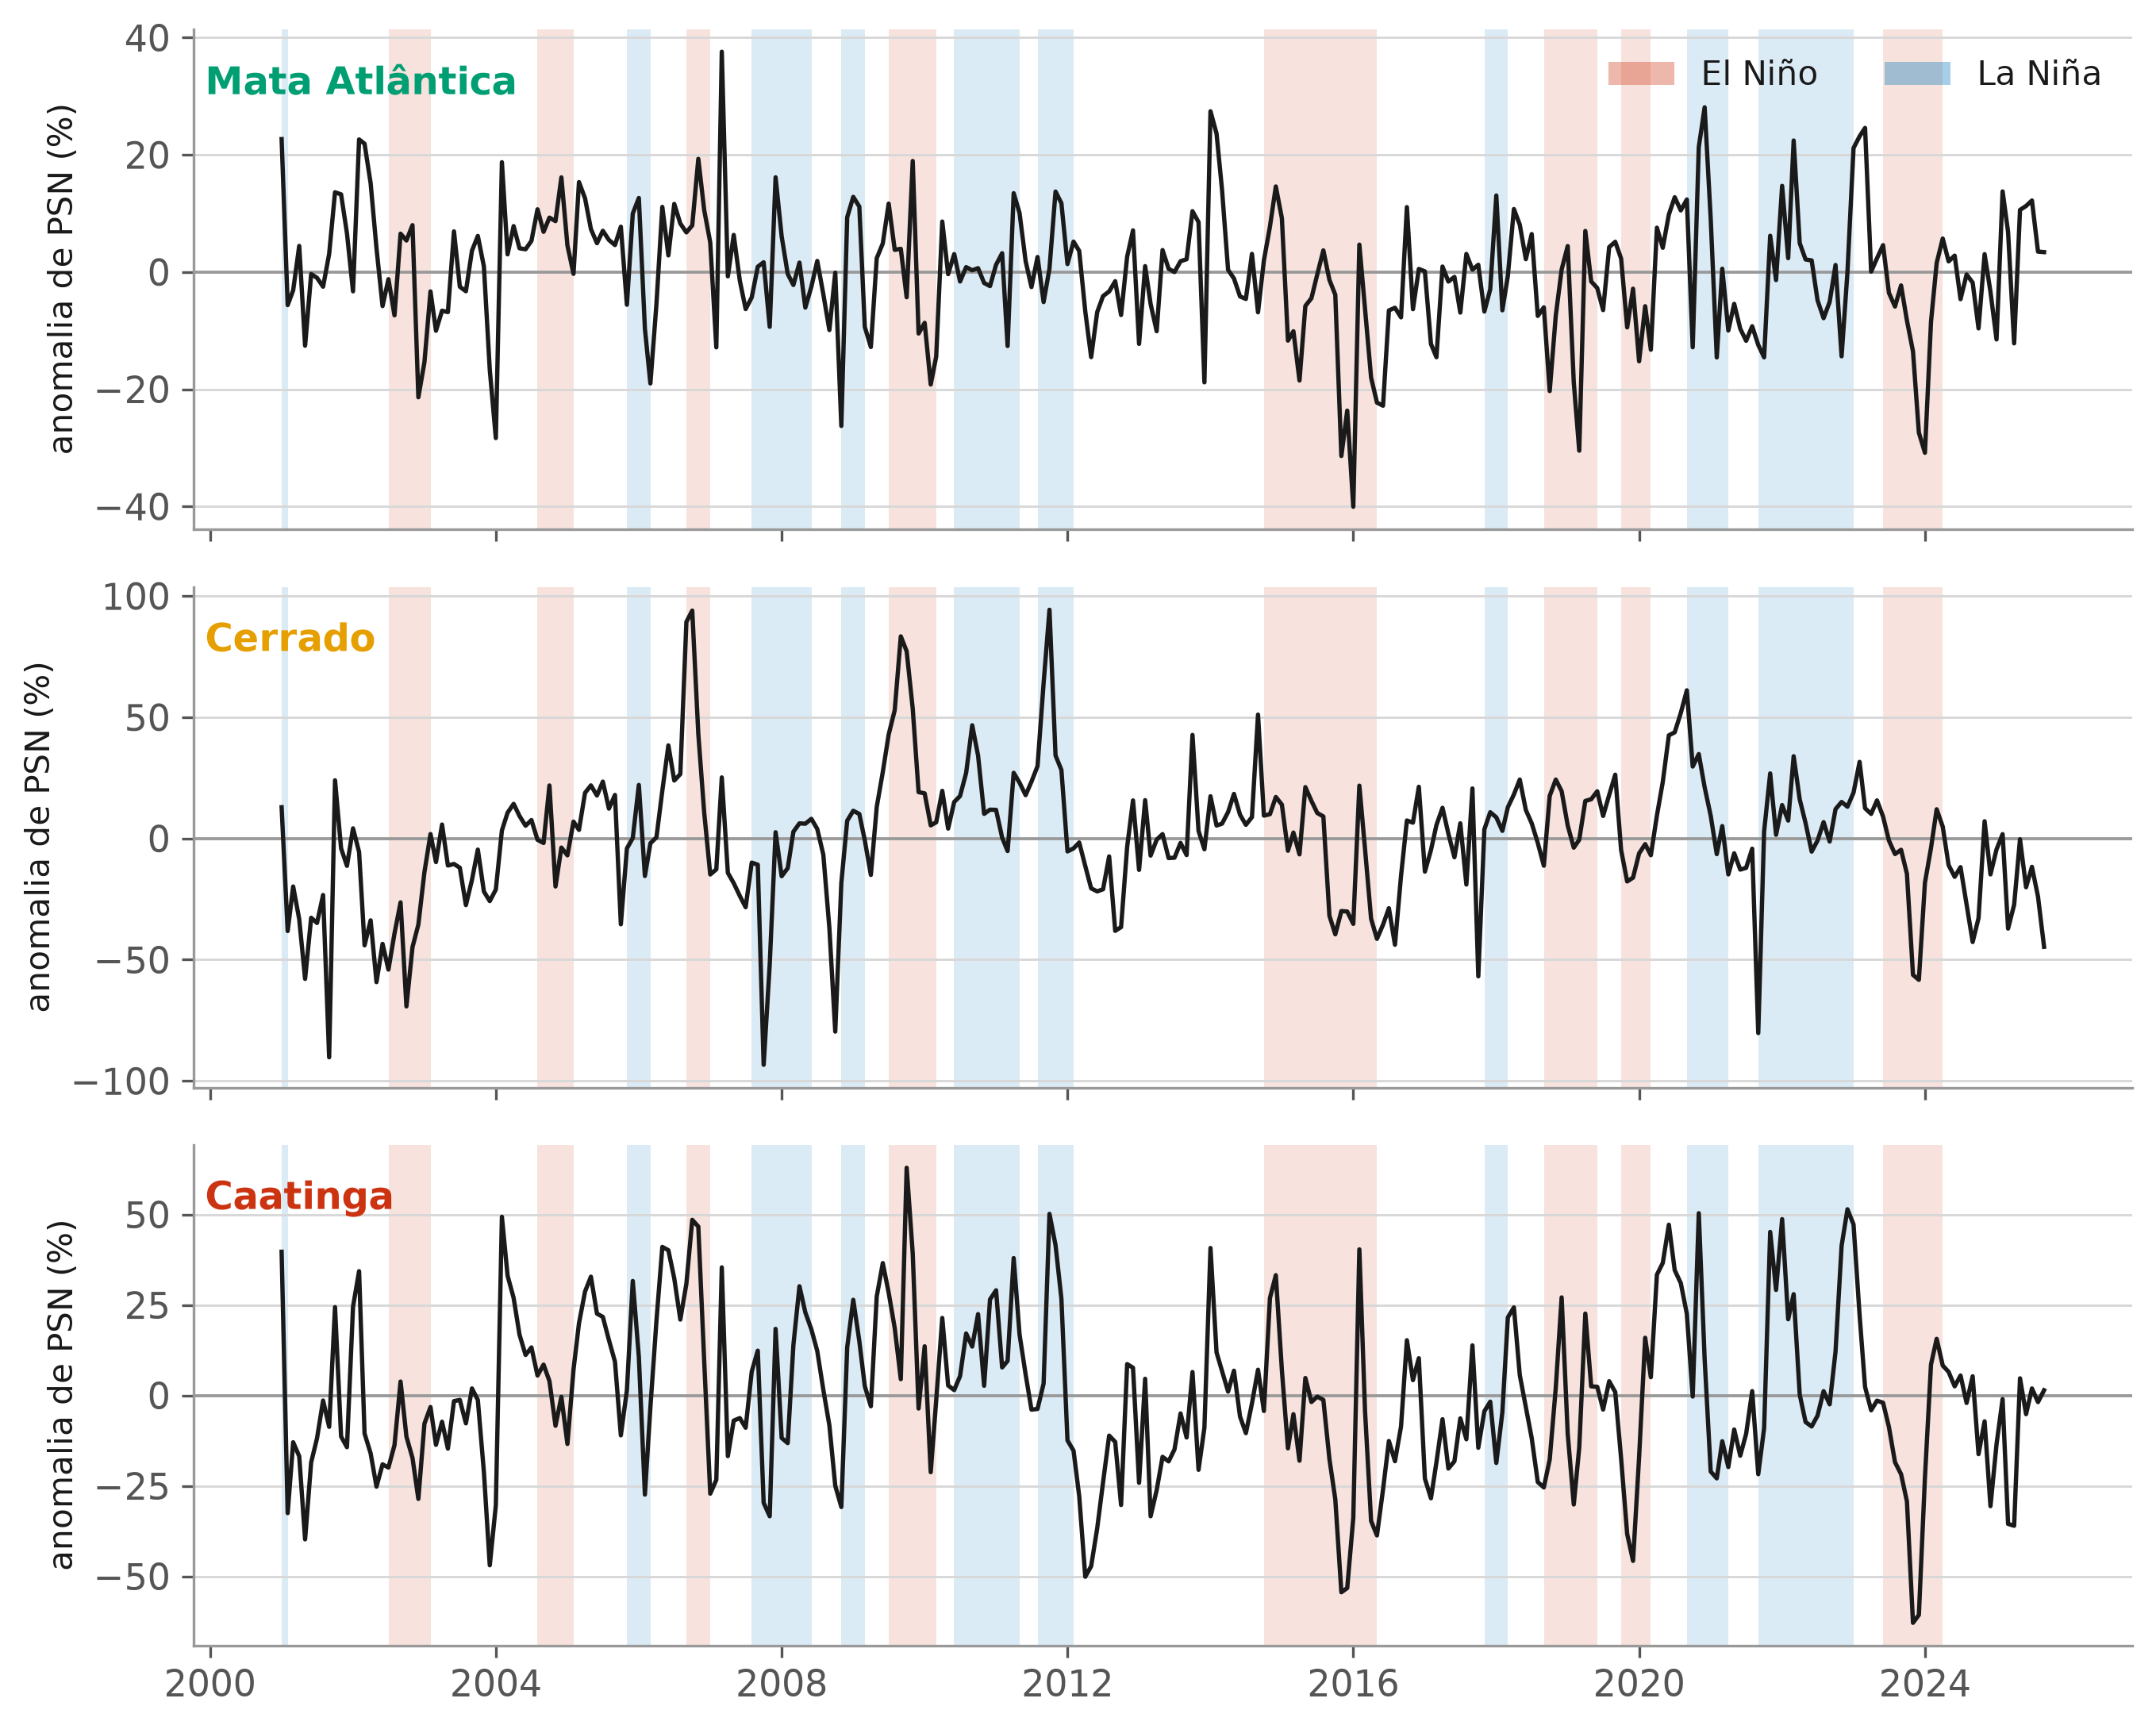
\includegraphics[width=\linewidth]{figs/fig1_episodios.png}
\caption{Anomalia percentual mensal da fotossíntese líquida nos três biomas entre 2001 e 2025, com os episódios de El Niño e de La Niña sombreados. As escalas verticais diferem entre os painéis.}
\label{fig:episodios}
\end{figure}

\subsection{Resposta da Mata Atlântica ao El Niño}

Na Mata Atlântica, a variável mais sensível às fases do ENSO foi a temperatura da superfície: nos meses de El Niño ela ficou 3,1~p.p.\ acima do normal da época, cerca de 0,9~$^{\circ}$C ($p < 0{,}001$), com 25\% desses meses no decil mais quente da série contra 5\% dos meses neutros (Tabela~\ref{tab:convencional}). A evapotranspiração e a precipitação não diferiram na posição central.

A PSN acompanhou esse aquecimento com um deslocamento negativo modesto no centro da distribuição e uma alteração forte na cauda. As medianas brutas são praticamente iguais nas três fases (133,3, 134,3 e 133,8~gC~m$^{-2}$ por período), mas, removido o ciclo anual, os meses de El Niño apresentaram anomalia média de $-5{,}4$~p.p.\ ($p = 0{,}010$) e 22,4\% deles ficaram abaixo do percentil 10 da série, contra 4,7\% dos meses neutros e 8,3\% dos de La Niña ($p = 0{,}0004$). O mínimo observado sob El Niño (79,0~gC~m$^{-2}$) fica 15 unidades abaixo do mínimo dos meses neutros (94,4). Nesse bioma, portanto, o El Niño atua sobre a cauda inferior da distribuição mais do que sobre o seu centro, o que explica por que um teste de posição aplicado a valores brutos não detectaria efeito. A La Niña não produziu resposta na Mata Atlântica em nenhuma das propriedades avaliadas ($-0{,}1$~p.p.; $p = 0{,}794$).

\begin{table*}[width=\textwidth,cols=7,pos=t]
\caption{Anomalia percentual média de cada fase ativa em relação aos meses neutros, com o valor de $p$ do teste de Mann-Whitney. Em negrito, os resultados que sobreviveram à correção de Benjamini-Hochberg (taxa de falsas descobertas de 5\%).}
\label{tab:convencional}
\begin{tabular*}{\tblwidth}{@{}llrrrr@{}}
\toprule
Bioma & Variável & \multicolumn{2}{c}{El Niño} & \multicolumn{2}{c}{La Niña} \\
\cmidrule(lr){3-4}\cmidrule(l){5-6}
 & & $\Delta$ (p.p.) & $p$ & $\Delta$ (p.p.) & $p$ \\
\midrule
Mata Atlântica & PSN & $\mathbf{-5{,}44}$ & \textbf{0,010} & $-0{,}08$ & 0,794 \\
               & EV  & $-1{,}52$ & 0,488 & $+1{,}37$ & 0,359 \\
               & PRE & $-5{,}28$ & 0,181 & $-1{,}27$ & 0,888 \\
               & TST & $\mathbf{+3{,}07}$ & \textbf{$<$0,001} & $-0{,}50$ & 0,322 \\
               & WAI & $-2{,}49$ & 0,189 & $+2{,}44$ & 0,182 \\
\addlinespace
Cerrado        & PSN & $+5{,}26$ & 0,375 & $\mathbf{+11{,}75}$ & \textbf{0,001} \\
               & EV  & $+7{,}51$ & 0,080 & $\mathbf{+10{,}22}$ & \textbf{$<$0,001} \\
               & PRE & $+7{,}91$ & 0,875 & $-7{,}73$ & 0,461 \\
               & TST & $+1{,}35$ & 0,217 & $-1{,}11$ & 0,050 \\
               & WAI & $+7{,}70$ & 0,245 & $\mathbf{+13{,}99}$ & \textbf{$<$0,001} \\
\addlinespace
Caatinga       & PSN & $-3{,}28$ & 0,458 & $\mathbf{+10{,}45}$ & \textbf{0,002} \\
               & EV  & $+0{,}34$ & 0,630 & $\mathbf{+10{,}85}$ & \textbf{0,003} \\
               & PRE & $+2{,}54$ & 0,761 & $+4{,}69$ & 0,837 \\
               & TST & $+1{,}51$ & 0,105 & $\mathbf{-2{,}14}$ & \textbf{0,013} \\
               & WAI & $+0{,}43$ & 0,534 & $\mathbf{+12{,}47}$ & \textbf{0,002} \\
\bottomrule
\end{tabular*}
\end{table*}

\subsection{Resposta do Cerrado e da Caatinga à La Niña}

Nos dois biomas sazonais a assimetria inverteu-se. No Cerrado, os meses de La Niña apresentaram evapotranspiração 10,2~p.p.\ acima do normal da época e disponibilidade hídrica 13,9~p.p.\ acima (ambos $p < 0{,}001$), enquanto nos meses de El Niño as anomalias correspondentes não foram significativas. A PSN respondeu no mesmo sentido, com anomalia média de $+11{,}7$~p.p.\ em La Niña ($p = 0{,}001$) e de $+5{,}3$~p.p.\ em El Niño ($p = 0{,}375$). O efeito da fase fria desloca a distribuição inteira: o primeiro quartil sobe de 65,1 para 85,8~gC~m$^{-2}$ por período.

Na Caatinga o padrão repetiu-se, com evapotranspiração 10,9~p.p.\ acima do normal em La Niña ($p = 0{,}003$), temperatura 2,1~p.p.\ abaixo ($p = 0{,}013$) e PSN 10,4~p.p.\ acima ($p = 0{,}002$; mediana de 94,6 contra 82,4~gC~m$^{-2}$ nos meses neutros). Nos meses de El Niño a PSN ficou 3,3~p.p.\ abaixo do normal, diferença não significativa ($p = 0{,}458$), ainda que 14,5\% desses meses tenham caído no decil mais baixo, contra 10,1\% dos neutros e 5,6\% dos de La Niña.

A precipitação do próprio mês não apresentou diferença significativa entre fases em nenhum bioma. As médias brutas sugeririam o contrário --- no Cerrado, 123~mm por período em La Niña e 107~mm em El Niño, contra 59~mm nos meses neutros ---, mas, como as duas fases ativas superam a neutra na mesma direção, trata-se do efeito de calendário antecipado na Seção~2.3: a diferença de 64~mm entre La Niña e meses neutros cai para 8~mm quando o ciclo anual é removido. O sinal do ENSO sobre a produtividade desses biomas aparece, portanto, nas variáveis que integram a água efetivamente utilizada pela vegetação, não no total precipitado no mês.

\subsection{Defasagem da resposta}

As correlações entre o ONI e a anomalia de PSN são negativas em todas as defasagens e em todos os biomas --- El Niño reduz e La Niña eleva a PSN ---, com magnitude entre 0,03 e 0,19 (Figura~\ref{fig:defasagem}). A defasagem de maior correlação difere entre os biomas: a Caatinga responde em fase, com o máximo em $L = 0$ ($\rho = -0{,}19$); a Mata Atlântica, com dois meses de atraso ($\rho = -0{,}16$); e o Cerrado, com dez meses ($\rho = -0{,}16$), permanecendo a correlação praticamente constante entre $L = 1$ e $L = 12$. A resposta do bioma semiárido é, portanto, imediata e de curta duração, e a do Cerrado, persistente --- um contraste compatível com a dinâmica de pulsos de recursos dos ecossistemas semiáridos \citep{schwinning2004} e com a integração da água no solo ao longo de semanas nos sistemas de savana \citep{oliveira2005}. Mesmo nos máximos, o coeficiente ao quadrado não ultrapassa 3,6\% da variância das anomalias.

\begin{figure}[pos=h]
\centering
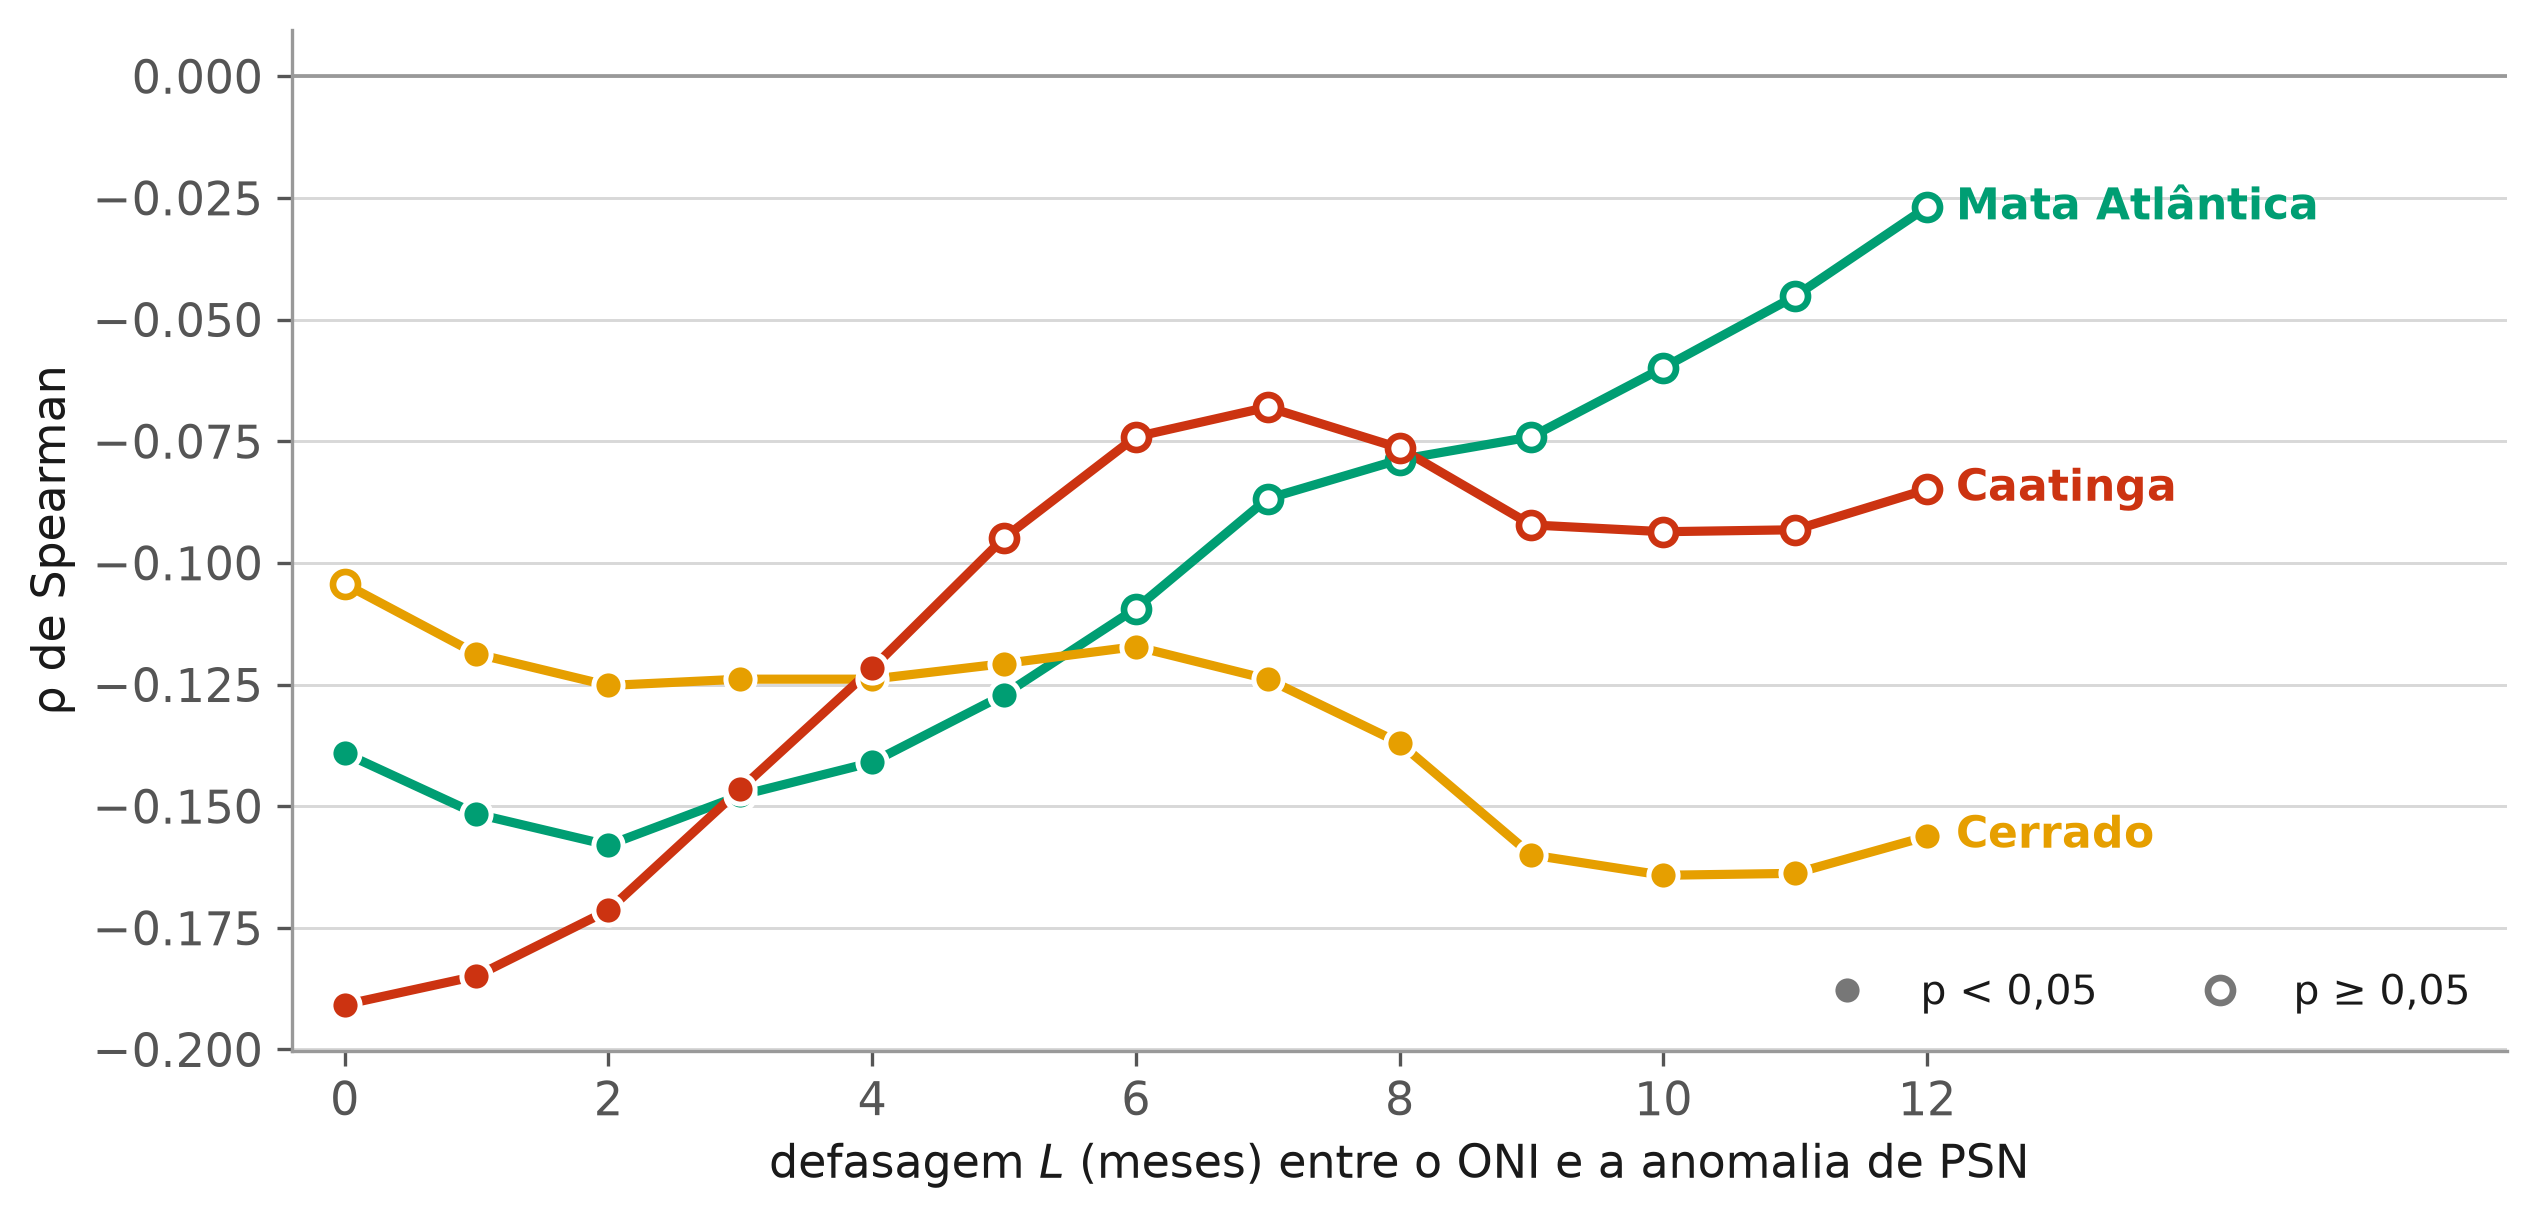
\includegraphics[width=\linewidth]{figs/fig3_defasagem.png}
\caption{Correlação de Spearman entre o ONI do mês $t$ e a anomalia de PSN do mês $t+L$. Os símbolos preenchidos indicam $p < 0{,}05$ sob a premissa de meses independentes.}
\label{fig:defasagem}
\end{figure}

\subsection{Mediação pelo modelo climático}

Impondo ao modelo de regressão polinomial as anomalias médias observadas em cada fase, a resposta predita da PSN reproduz boa parte da observada nas combinações de maior magnitude (Tabela~\ref{tab:mediacao}). Na Caatinga em La Niña, o modelo prediz $+9{,}8\%$ contra $+10{,}4\%$ observados, isto é, 94\% da resposta; no Cerrado na mesma fase, $+8{,}0\%$ contra $+11{,}7\%$, ou 68\%; e na Mata Atlântica em El Niño, $-3{,}1\%$ contra $-5{,}4\%$, ou 57\%. A decomposição por preditor mostra que a via difere entre os biomas: deslocar apenas a evapotranspiração já produz $+11{,}6\%$ no Cerrado e $+9{,}0\%$ na Caatinga, ao passo que na Mata Atlântica a temperatura sozinha responde por $-2{,}8\%$ dos $-3{,}1\%$ preditos. O clima medido reproduz, assim, a maior parte da resposta nos biomas sazonais e pouco mais da metade no bioma úmido.

\begin{table}[width=\linewidth,cols=5,pos=h]
\caption{Resposta da PSN predita pelo modelo climático quando lhe são impostas as anomalias médias de cada fase, comparada à observada. A coluna final é a razão entre as duas.}
\label{tab:mediacao}
\begin{tabular*}{\tblwidth}{@{}llrrr@{}}
\toprule
Bioma & Fase & Predito (\%) & Observado (\%) & Razão \\
\midrule
Mata Atlântica & El Niño & $-3{,}11$ & $-5{,}44$  & 0,57 \\
Mata Atlântica & La Niña & $+0{,}74$ & $-0{,}08$  & --- \\
Cerrado        & El Niño & $+4{,}48$ & $+5{,}26$  & 0,85 \\
Cerrado        & La Niña & $+8{,}02$ & $+11{,}75$ & 0,68 \\
Caatinga       & El Niño & $-1{,}17$ & $-3{,}28$  & 0,36 \\
Caatinga       & La Niña & $+9{,}84$ & $+10{,}45$ & 0,94 \\
\bottomrule
\end{tabular*}
\end{table}

\subsection{Variabilidade interanual}

Nenhum dos três biomas apresentou tendência significativa da PSN anual entre 2001 e 2024 (Tabela~\ref{tab:interanual}). O declive de Sen foi negativo na Mata Atlântica ($-4{,}3$~gC~m$^{-2}$~ano$^{-1}$, equivalente a $-6{,}2\%$ no período) e positivo no Cerrado ($+11{,}3\%$) e na Caatinga ($+0{,}7\%$), mas os intervalos de confiança cruzam zero em todos os casos ($p = 0{,}070$, 0,333 e 0,941). Como verificação de consistência, a soma anual de PSN foi comparada ao NPP anual do produto MOD17A3HGF para as mesmas máscaras de bioma, com correlação de Pearson entre 0,993 e 0,999 nos três casos.

A variabilidade interanual é muito desigual entre os biomas: o coeficiente de variação da PSN anual é de 4,6\% na Mata Atlântica, contra 15,0\% no Cerrado e 13,3\% na Caatinga. Os anos extremos não coincidem com as fases do ENSO de forma sistemática. O pior ano da Mata Atlântica, 2016 (1.448~gC~m$^{-2}$~ano$^{-1}$), sucede o El Niño de 2014--2016, mas o melhor ano do Cerrado, 2009 (1.407~gC~m$^{-2}$~ano$^{-1}$), é também um ano de El Niño, e o melhor da Caatinga, 2020 (1.276~gC~m$^{-2}$~ano$^{-1}$), é um ano neutro. A escala anual mistura meses de fases distintas e é, por isso, menos nítida do que a análise mensal em anomalias.

\begin{table}[width=\linewidth,cols=6,pos=h]
\caption{Variabilidade interanual da PSN entre 2001 e 2024. O declive de Sen é expresso em porcentagem do período e testado por Mann-Kendall.}
\label{tab:interanual}
\begin{tabular*}{\tblwidth}{@{}lrrrrr@{}}
\toprule
Bioma & Média & CV & Sen & $p$ & Extremos \\
 & (gC~m$^{-2}$~ano$^{-1}$) & (\%) & (\%) & & (mín/máx) \\
\midrule
Mata Atlântica & 1.604 & 4,6  & $-6{,}2$  & 0,070 & 2016/2014 \\
Cerrado        & 1.157 & 15,0 & $+11{,}3$ & 0,333 & 2002/2009 \\
Caatinga       & 1.044 & 13,3 & $+0{,}7$  & 0,941 & 2012/2020 \\
\bottomrule
\end{tabular*}
\end{table}

\subsection{Robustez: o episódio como unidade amostral}

Repetindo o cálculo com o episódio como unidade, o sentido e a magnitude das respostas não mudam --- a estatística $\Delta$ é a mesma ---, mas a precisão com que elas são estimadas diminui de forma apreciável. A largura mediana do intervalo de confiança passa de 12,9 para 23,1 pontos percentuais, um alargamento de 1,67 vez em mediana, que chega a 2,53 vezes no Cerrado em El Niño. Dos 30 testes, 10 tinham intervalo excluindo o zero com o mês como unidade e 3 o mantêm com o episódio (Tabela~\ref{tab:unidade}, Figura~\ref{fig:unidade}).

\begin{table*}[width=\textwidth,cols=8,pos=t]
\caption{Os dez efeitos cujo intervalo de confiança exclui o zero com o mês como unidade, recalculados com o episódio como unidade amostral. $\Delta$ é a mesma estatística nos dois esquemas; o que muda é a reamostragem. Em negrito, os três que permanecem.}
\label{tab:unidade}
\begin{tabular*}{\tblwidth}{@{}lllrrrrr@{}}
\toprule
 & & & & \multicolumn{2}{c}{Mês como unidade} & \multicolumn{2}{c}{Episódio como unidade} \\
\cmidrule(lr){5-6}\cmidrule(l){7-8}
Bioma & Var. & Fase & $\Delta$ (p.p.) & IC95\% & $p$ & IC95\% & $p$ \\
\midrule
Mata Atlântica & PSN & El Niño & $-5{,}44$  & $-8{,}7$ a $-2{,}3$ & 0,001 & $\mathbf{-9{,}2}$ \textbf{a} $\mathbf{-0{,}05}$ & \textbf{0,048} \\
Mata Atlântica & TST & El Niño & $+3{,}07$  & $+1{,}7$ a $+4{,}4$ & $<0{,}001$ & $\mathbf{+0{,}9}$ \textbf{a} $\mathbf{+5{,}3}$ & \textbf{0,005} \\
Caatinga       & PSN & La Niña & $+10{,}45$ & $+4{,}4$ a $+16{,}4$ & 0,001 & $\mathbf{+0{,}4}$ \textbf{a} $\mathbf{+16{,}9}$ & \textbf{0,044} \\
\addlinespace
Cerrado        & PSN & La Niña & $+11{,}75$ & $+4{,}3$ a $+18{,}9$ & 0,003 & $-1{,}5$ a $+24{,}3$ & 0,081 \\
Cerrado        & WAI & La Niña & $+13{,}99$ & $+6{,}8$ a $+21{,}1$ & $<0{,}001$ & $-2{,}6$ a $+27{,}9$ & 0,087 \\
Cerrado        & EV  & La Niña & $+10{,}22$ & $+4{,}3$ a $+15{,}8$ & 0,001 & $-3{,}5$ a $+21{,}5$ & 0,135 \\
Cerrado        & EV  & El Niño & $+7{,}51$  & $+0{,}6$ a $+14{,}5$ & 0,031 & $-6{,}8$ a $+23{,}2$ & 0,322 \\
Caatinga       & WAI & La Niña & $+12{,}47$ & $+5{,}2$ a $+19{,}6$ & 0,001 & $-2{,}2$ a $+22{,}0$ & 0,086 \\
Caatinga       & EV  & La Niña & $+10{,}85$ & $+4{,}5$ a $+17{,}2$ & 0,001 & $-2{,}2$ a $+19{,}8$ & 0,103 \\
Caatinga       & TST & La Niña & $-2{,}14$  & $-3{,}7$ a $-0{,}6$ & 0,008 & $-5{,}2$ a $+2{,}1$ & 0,327 \\
\bottomrule
\end{tabular*}
\end{table*}

\begin{figure}[pos=h]
\centering
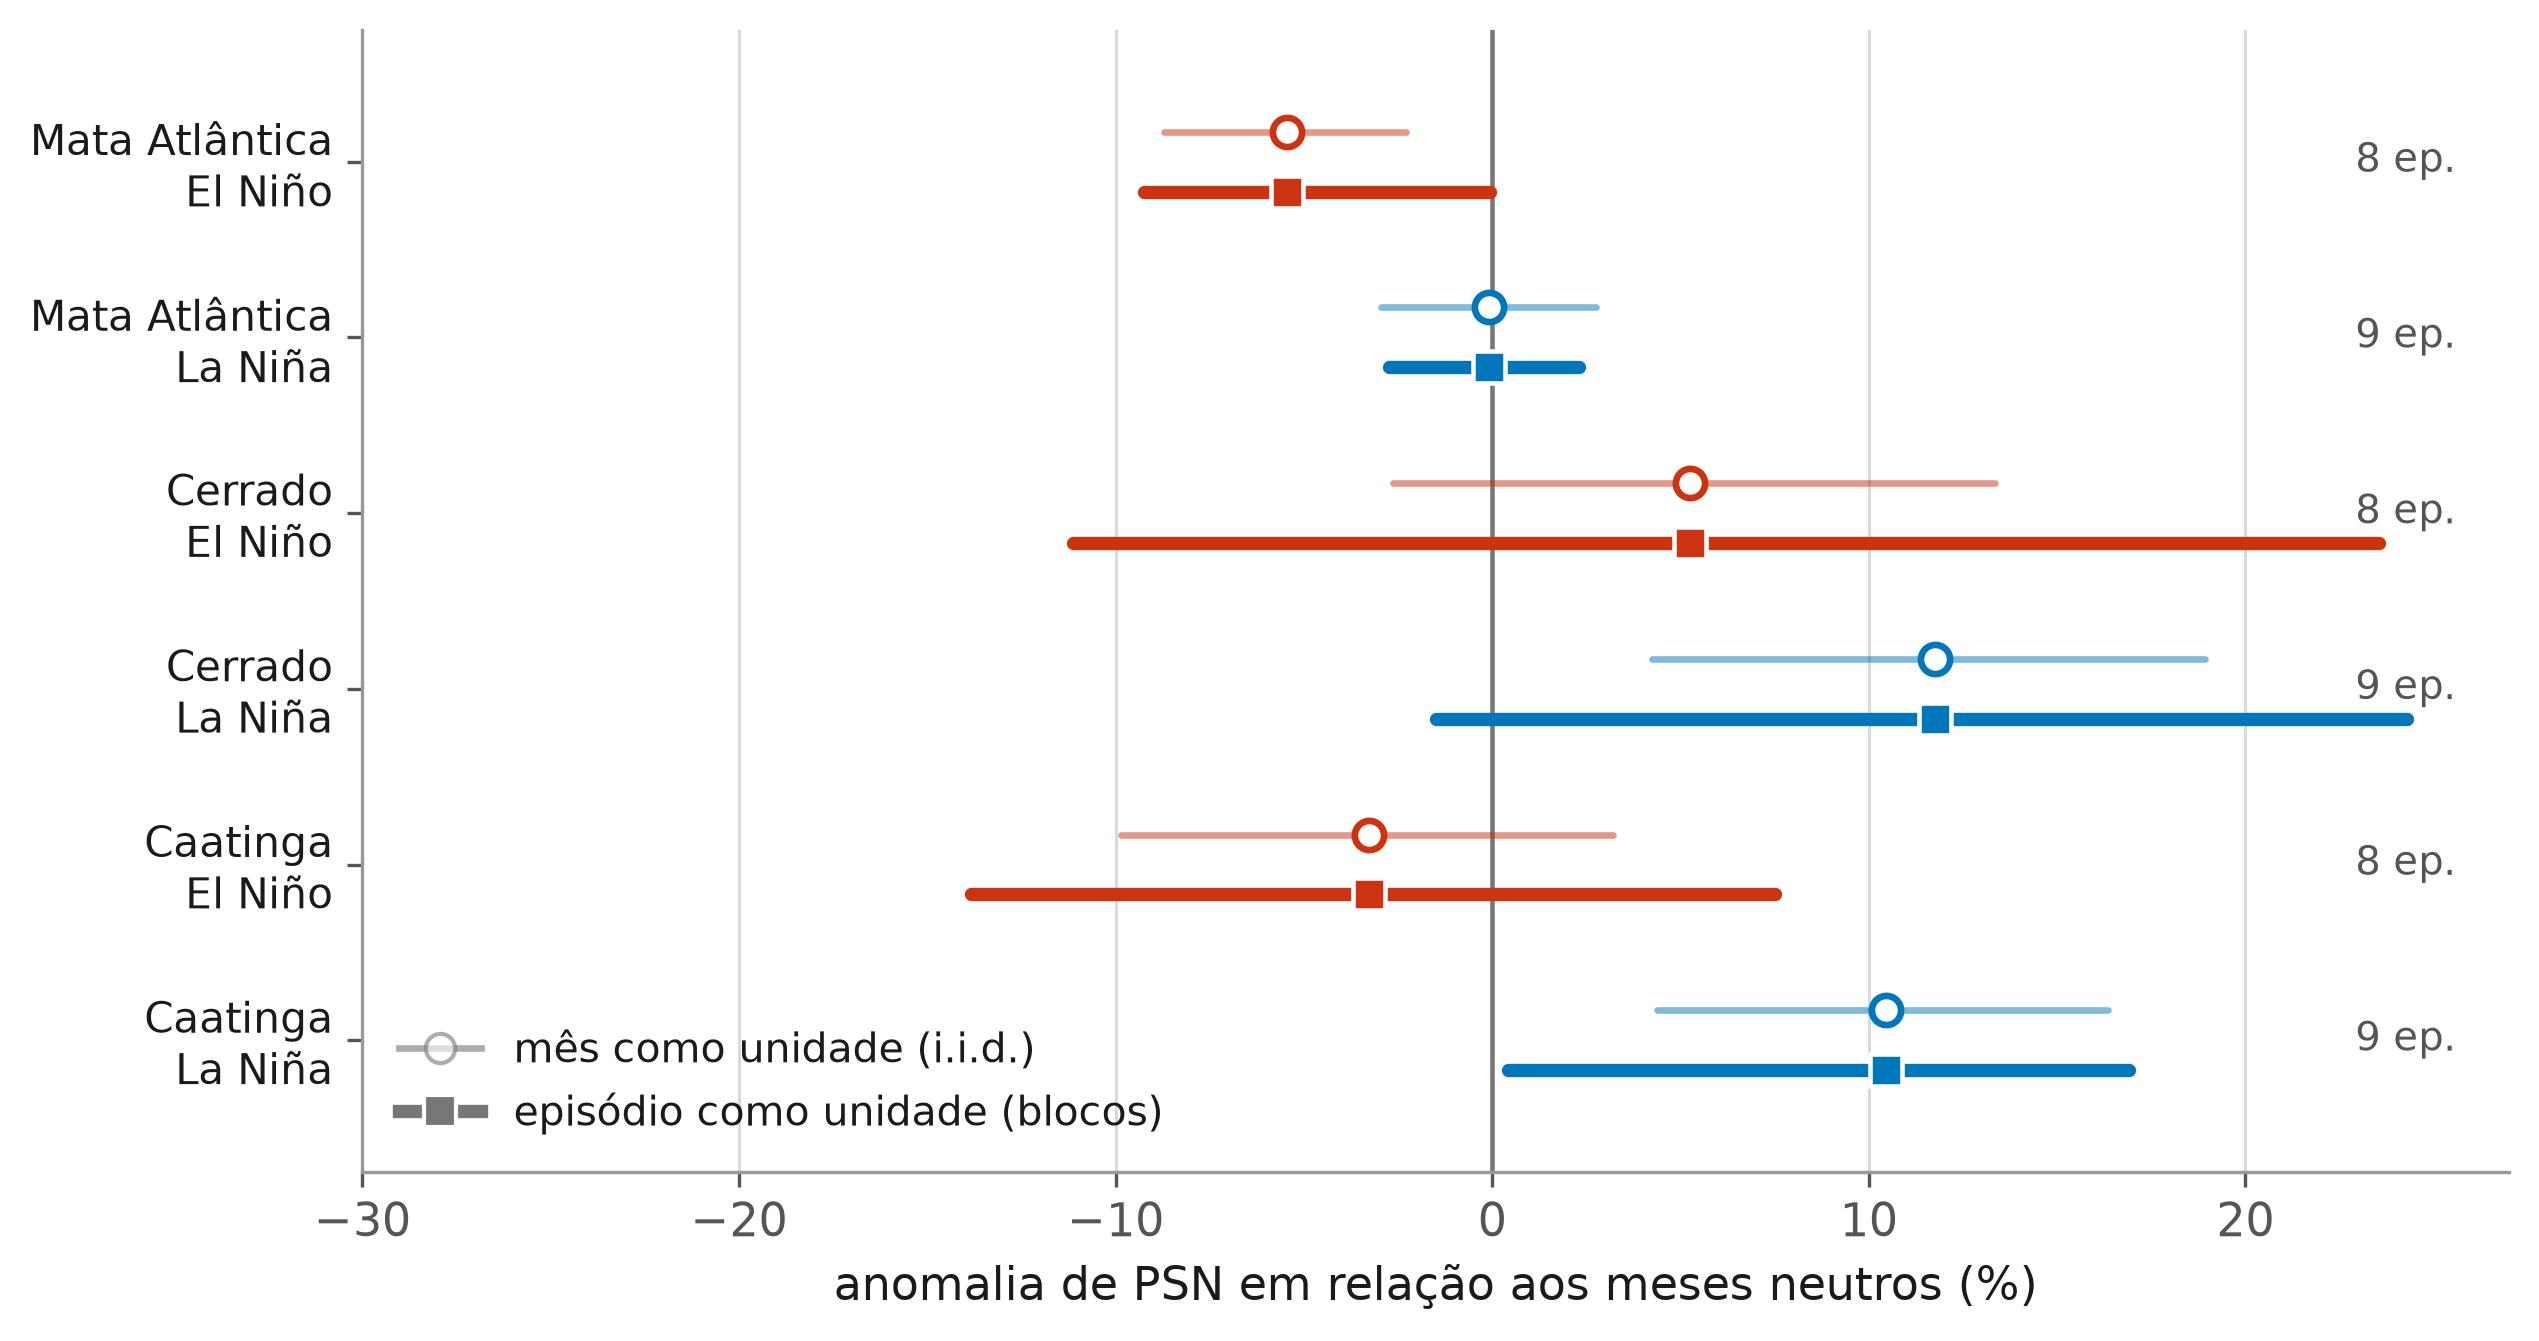
\includegraphics[width=\linewidth]{figs/fig2_unidade.png}
\caption{Anomalia de PSN de cada fase em relação aos meses neutros, com intervalos de confiança de 95\% obtidos por bootstrap sobre meses (linha fina, círculo aberto) e por bootstrap em blocos sobre episódios (linha grossa, quadrado). O número de episódios de cada fase consta à direita.}
\label{fig:unidade}
\end{figure}

Os três que permanecem são justamente os dois polos do gradiente: o aquecimento da superfície da Mata Atlântica em El Niño (IC95\% $+0{,}9$ a $+5{,}3$~p.p.; $p = 0{,}005$), o mais robusto do conjunto, a redução da PSN desse mesmo bioma e fase (IC95\% $-9{,}2$ a $-0{,}05$~p.p.; $p = 0{,}048$) e o aumento da PSN da Caatinga em La Niña (IC95\% $+0{,}4$ a $+16{,}9$~p.p.; $p = 0{,}044$). Os dois últimos são marginais. No Cerrado, o aumento de 11,7~p.p.\ da PSN em La Niña passa a $p = 0{,}081$, com intervalo de $-1{,}5$ a $+24{,}3$~p.p., quando as nove sequências de La Niña são tomadas como as nove observações que de fato são.

A assimetria descrita nas Seções~3.2 e 3.3 --- Mata Atlântica associada à fase quente, biomas sazonais à fase fria --- é, portanto, consistente entre os dois esquemas, e nenhum resultado troca de sinal. O que a verificação mostra é que a magnitude de cada efeito é estimada com precisão limitada pelo número de episódios disponíveis, e não pelo número de meses.

\section{Discussão}

Os três biomas respondem ao mesmo forçante remoto de maneiras distintas, e a diferença acompanha o fator que limita a produtividade de cada um. Na Mata Atlântica, onde a água raramente é limitante, o canal é térmico: o El Niño eleva a temperatura da superfície em cerca de 0,9~$^{\circ}$C e a produtividade cai, sobretudo pela multiplicação dos meses extremamente baixos. A sensibilidade da fotossíntese à demanda evaporativa em florestas tropicais úmidas \citep{lawson2019, vourlitis2022} e o fato de a teleconexão do ENSO com o Leste do Nordeste brasileiro ser mais consistente na temperatura do que na precipitação \citep{ropelewski1987, kayano2007} tornam esse resultado esperado. No Cerrado e na Caatinga, limitados pela água, o canal é hídrico e o sinal aparece na fase fria, quando o excedente de água disponível eleva a evapotranspiração e, com ela, a assimilação de carbono.

Que o sinal apareça na evapotranspiração e na disponibilidade hídrica, e não na precipitação do próprio mês, é coerente com a fisiologia envolvida: transpiração e assimilação ocorrem pelos mesmos estômatos \citep{lawson2019}, de modo que a água efetivamente utilizada informa sobre a produtividade melhor do que o total que caiu no mês. A precipitação é um fluxo de entrada ruidoso, e a vegetação responde à água que permaneceu disponível no solo nas semanas seguintes \citep{oliveira2005, schwinning2004}. A defasagem observada reforça esse quadro: a Caatinga responde no próprio mês, à maneira de um sistema de pulsos \citep{schwinning2004, mendes2020}, enquanto no Cerrado a correlação permanece estável por até doze meses, compatível com a integração da água em profundidade nas savanas \citep{oliveira2005, bucci2008}.

A mediação pelo modelo climático quantifica até onde o clima medido leva. Nos biomas sazonais, de 68\% a 94\% da resposta é reproduzida pelo deslocamento dos preditores, quase inteiramente pela evapotranspiração; no bioma úmido, pouco mais da metade, sobretudo pela temperatura. A parcela restante não é explicada pelos preditores do mesmo mês e pode envolver radiação, defasagem da resposta e, na Mata Atlântica, variáveis estruturais da paisagem que não compõem o modelo \citep{broggio2024, ribeiro2009}.

A verificação de robustez qualifica o alcance dessas afirmações sem alterar sua direção. Em 24 anos há 8 episódios de El Niño e 9 sequências de La Niña; blocos de duração mediana próxima a 8 meses fazem o tamanho amostral efetivo ser uma fração do nominal, e o erro-padrão cresce aproximadamente com a raiz dessa razão. O alargamento mediano de 1,67 vez é o que se esperaria dessa aritmética, e não um efeito peculiar a esta série: ele deve aparecer sempre que compósitos de fase forem montados sobre observações mensais de episódios plurianuais. A implicação prática é que diferenças de poucos pontos percentuais entre fases dificilmente se sustentam com séries dessa extensão, e que a evidência mais sólida aqui obtida --- os dois polos do gradiente --- é também a que envolve os efeitos de maior magnitude.

Algumas limitações devem ser explicitadas. O bootstrap em blocos com 8 ou 9 blocos é ele próprio impreciso: intervalos percentílicos construídos sobre tão poucas unidades têm cobertura apenas aproximada, e os valores de $p$ marginais reportados devem ser lidos como indicativos. A classificação em três fases descarta a intensidade dos episódios, que varia de um ONI de pico de 0,71 a 2,59 na série. A análise é correlacional e não separa o efeito do ENSO de outros modos de variabilidade que possam coincidir com ele no período, como a Oscilação Decadal do Pacífico \citep{kayano2007}. A PSN e a evapotranspiração provêm de algoritmos MODIS que compartilham entradas, de modo que a mediação não constitui evidência independente. Por fim, a temperatura da superfície não passou por filtro de qualidade pela banda QC\_Day, e a sensibilidade da série a esse filtro não foi avaliada.

Duas direções decorrem do exposto. A primeira é estender a série para trás do início do registro MODIS, por produtos de sensores anteriores ou por reconstruções, ou aumentar a replicação espacial analisando sub-regiões dentro de cada bioma, de modo a elevar o número de unidades independentes disponíveis. A segunda é metodológica: compósitos de fase do ENSO construídos sobre séries mensais ganham em transparência quando acompanhados de alguma forma de inferência que respeite a estrutura temporal --- bootstrap em blocos, testes de permutação sobre rótulos de episódio ou correção do tamanho amostral efetivo \citep{kunsch1989, politis1994} ---, cujo custo computacional é baixo.

\section{Conclusões}

A fotossíntese líquida dos três biomas da Bahia responde às fases do ENSO de forma assimétrica e específica de cada bioma. A Mata Atlântica responde à fase quente, com redução média de 5,4~p.p.\ e multiplicação por quase cinco da frequência de meses extremamente baixos, acompanhando um aquecimento da superfície de cerca de 0,9~$^{\circ}$C. O Cerrado e a Caatinga respondem à fase fria, com aumentos de 11,7 e 10,4~p.p., acompanhados de anomalias positivas de evapotranspiração e de disponibilidade hídrica, e não do total precipitado no mês. O modelo climático reproduz de 57\% a 94\% da magnitude observada, pela via térmica no bioma úmido e pela hídrica nos sazonais, e a defasagem da resposta vai de zero meses na Caatinga a dez no Cerrado. Nenhum bioma apresenta tendência interanual significativa no período.

Quando a unidade amostral passa do mês para o episódio, o padrão assimétrico se mantém e nenhum resultado troca de sinal, mas os intervalos de confiança alargam-se 1,67 vez em mediana e permanecem distinguíveis de zero apenas três efeitos, entre os quais os dois polos do gradiente. Os resultados caracterizam, portanto, três regimes distintos de associação entre o ENSO e a produtividade, e indicam que sua magnitude deve ser reportada com a precisão que o número de episódios --- e não o de meses --- permite.

\section*{Disponibilidade de dados}
A base mensal (297 períodos por bioma, 2001--2025), o código em Python de todas as análises aqui reportadas e os resultados da rodada completa estão disponíveis em \url{https://github.com/heroslore/MRMP-N-PSN-Bahia} e arquivados de forma permanente no Zenodo sob o DOI \url{https://doi.org/10.5281/zenodo.22883915}, que resolve sempre para a versão mais recente do arquivo. A base é também fornecida como material suplementar (arquivo CSV).

\section*{Declaração de conflito de interesses}
Os autores declaram não haver conflitos de interesse financeiros ou pessoais que pudessem ter influenciado o trabalho relatado neste artigo.

\section*{Agradecimentos}
O presente trabalho foi realizado com apoio da Coordenação de Aperfeiçoamento de Pessoal de Nível Superior -- Brasil (CAPES) -- Código de Financiamento 001, por meio de bolsa de mestrado concedida ao primeiro autor. Os autores agradecem ao Programa de Pós-graduação em Ciências e Tecnologias Ambientais (UFSB/IFBA). O primeiro autor agradece ao Prof. Dr. Fabrício Berton Zanchi, pela orientação, e à Profa. Dra. Nayanne Silva Benfica, pela coorientação.

\section*{CRediT authorship contribution statement}
\textbf{Ygor Augusto dos Santos Oliveira:} Conceituação, Metodologia, Software, Análise formal, Curadoria de dados, Redação -- rascunho original. \textbf{Nayanne Silva Benfica:} Conceituação, Metodologia, Curadoria de dados, Redação -- revisão e edição, Supervisão. \textbf{Fabrício Berton Zanchi:} Conceituação, Metodologia, Redação -- revisão e edição, Supervisão.

\bibliographystyle{cas-model2-names}
\bibliography{refs2}

\end{document}
